\documentclass[11pt]{article}
\usepackage[scaled=0.92]{helvet}
\usepackage{geometry}
\geometry{letterpaper,tmargin=1in,bmargin=1in,lmargin=1in,rmargin=1in}
\usepackage[parfill]{parskip} % Activate to begin paragraphs with an empty line rather than an indent %\usepackage{graphicx}
\usepackage{amsmath,amssymb, mathrsfs, dsfont}
\usepackage{tabularx}
\usepackage[font=footnotesize,labelfont=bf]{caption}
\usepackage{graphicx}
\usepackage{xcolor}
%\usepackage[linkbordercolor ={1 1 1} ]{hyperref}
%\usepackage[sf]{titlesec}
\usepackage{natbib}
\usepackage{../../Tianpei_Report}


\begin{document}
\title{Self-study: Entropic regularization of optimal transport}
\author{ Tianpei Xie}
\date{ Aug. 17th., 2022 }
\maketitle
\tableofcontents
\newpage
\section{Recall: Optimal transport problem}
Recall the problem of optimal transport:
\begin{itemize}
\item The \textbf{primal problem} for discrete measures, $\alpha = \sum_{i=1}^{n}a_i \delta_{\mb{x}_{i}}$ and $\beta := \sum_{i=1}^{m}b_i \delta_{\mb{y}_{i}}$, 
\begin{align}
\min_{\mb{P} \in \bR_{+}^{n \times m}} & \inn{\mb{P}}{\mb{C}} = \sum_{i,j}C_{i,j} P_{i,j} \label{eqn: optimal_transport_primal}\\
\text{s.t. }&  \mb{P}\mb{1}_{m} = \mb{a} \nonumber\\
&\mb{P}^{T}\mb{1}_{n} = \mb{b}   \nonumber \\
&P_{i,j} \ge 0 \nonumber
\end{align} where $\mb{C}_{n,m} := [C_{i,j}]_{i\in [1:n], j\in [1:m]}$,  $C_{i,j}:= c(\mb{x}_i, \mb{y}_j) \ge 0$. The feasible set is defined as
\begin{align}
U(\mb{a}, \mb{b}) := \set{\mb{P} \in \bR_{+}^{n \times m}: \mb{P}\mb{1}_{m} = \mb{a},\;\mb{P}^{T}\mb{1}_{n} = \mb{b}} \label{eqn: optimal_transport_feasible_set}
\end{align}

We can define 
\begin{align*}\mb{A} &= \left[
\begin{array}{c}
\mb{1}_{n}^{T}\otimes \mb{I}_{m} \\
\mb{I}_{n}\otimes  \mb{1}_{m}^{T}
\end{array}\right] 
=  \left[
\begin{array}{ccc}
 \mb{I}_{m}& \ldots & \mb{I}_{m}\\
 \mb{I}_{n} &  \ldots &\mb{I}_{n}
\end{array}
\right]_{nm \times nm}
\end{align*} and $\mb{p} = [P_{i*(m-1)+j}] \in \bR^{nm \times 1}$, and $\mb{c} = [C_{i*(m-1)+j}] \in \bR^{nm \times 1}$.
Then the primal problem can be writen in matrix form
\begin{align}
\min_{\mb{p} \in \bR_{+}^{nm \times 1}} & \mb{c}^{T}\mb{p} \label{eqn: optimal_transport_primal_mat}\\
\text{s.t. }&  \mb{A}\mb{p} = \left[
\begin{array}{c}
\mb{a} \\
\mb{b}
\end{array}\right]  \nonumber
\end{align}

\item The dual problem for optimal transport: 
\begin{align}
\max_{\mb{\lambda} \in \bR^{n}, \mb{\mu} \in \bR^{m}} & \inn{\mb{\lambda}}{\mb{a}} + \inn{\mb{\mu}}{\mb{b}} \label{eqn: optimal_transport_dual}\\
\text{s.t. } & \lambda_i + \mu_{j} \le C_{i,j}\quad \forall\, i\in [1:n], j\in [1:m] \nonumber
\end{align} where $\mb{\lambda}= [\lambda_i]_{n}$, $\mb{\mu}= [\mu_{j}]_{m}$ are \textbf{dual variables} (slack variables) for marginal distribution constrain $\mb{a}$ and $\mb{b}$. We denote $\mb{\lambda}\oplus \mb{\mu}:= \mb{\lambda}\mb{1}_{m}^{T} + \mb{1}_{n}\mb{\mu}^{T} \in \bR^{n\times m}$ so that the linear constraints is $\mb{\lambda}\oplus \mb{\mu} \le \mb{C}$. Such dual variables $\mb{\lambda}$, $\mb{\mu}$ are often referred to as "\emph{\textbf{Kantorovich potentials}}."  The feasible set of the dual problem is defined as 
\begin{align}
R(\mb{C}) := \set{\mb{\lambda} \in \bR^{n}, \mb{\mu} \in \bR^{m}: \mb{\lambda}\oplus \mb{\mu} \le \mb{C}} \label{eqn: optimal_transport_dual_feasible_set}
\end{align} where $\mb{\lambda}\oplus \mb{\mu} = \mb{\lambda}\mb{1}_{m} + \mb{1}_n \mb{\mu}^{T}.$

Similarly, we have the dual problem in matrix form, when we define $\mb{h} = \left[
\begin{array}{c}
\mb{\lambda} \\
\mb{\mu}
\end{array}\right] \in \bR^{nm \times 1}$

\begin{align}
\max_{\mb{h} \in \bR^{nm \times 1}} & \left[
\begin{array}{cc}
\mb{a}^{T} & \mb{b}^{T}
\end{array}\right]  \mb{h} \label{eqn: optimal_transport_dual_mat}\\
\text{s.t. }&  \mb{A}^{T}\mb{h} \le \mb{c} \nonumber
\end{align}
\end{itemize}





\section{Entropic regularization of optimal transport}
This section introduces a family of numerical schemes to approximate solutions to Kantorovich formulation of optimal transport and its many generalizations. It operates by adding an entropic regularization penalty to the original problem. This regularization has several important advantages:
\begin{itemize}
\item the minimization of the regularized problem can be solved using a simple \emph{alternate minimization} scheme, which only required matrix-vector multiplication, 

\item the resulting approximate distance is \emph{smooth} with respect to input histogram weights and positions of the Diracs and can be differentiated using \emph{automatic differentiation}.
\end{itemize}

\subsection{Entropic regularization}
We introduce addtional entropic regularization term to the primal problem \eqref{eqn: optimal_transport_primal}:
\begin{align}
H(\mb{P}) &:= -\sum_{i,j}P_{i,j}\paren{\log(P_{i,j}) - 1} \label{eqn: entropy_regularization}
\end{align} The function $H$ is \emph{\textbf{$1$-strongly concave}}, because its Hessian is $\partial^2 H(\mb{P}) = −\diag{1/P_{i,j}} > 0$ and $P_{i,j} \le 1$. 

\begin{figure}
\begin{minipage}[t]{1\linewidth}
  \centering
  \centerline{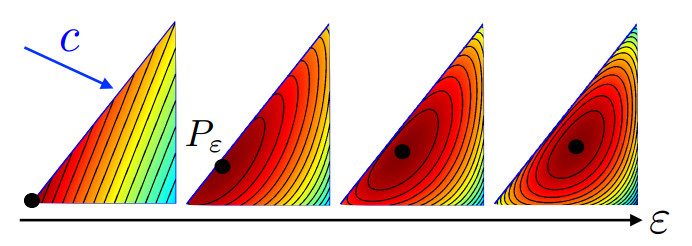
\includegraphics[scale = 0.4]{entropy_regularization1.png}}
\end{minipage}
\caption{\footnotesize{\textbf{The effect of entropy regularization is to diffuse the results.}}}
\label{fig: entropy_regularization1}
\end{figure}
\begin{figure}
\begin{minipage}[t]{1\linewidth}
  \centering
  \centerline{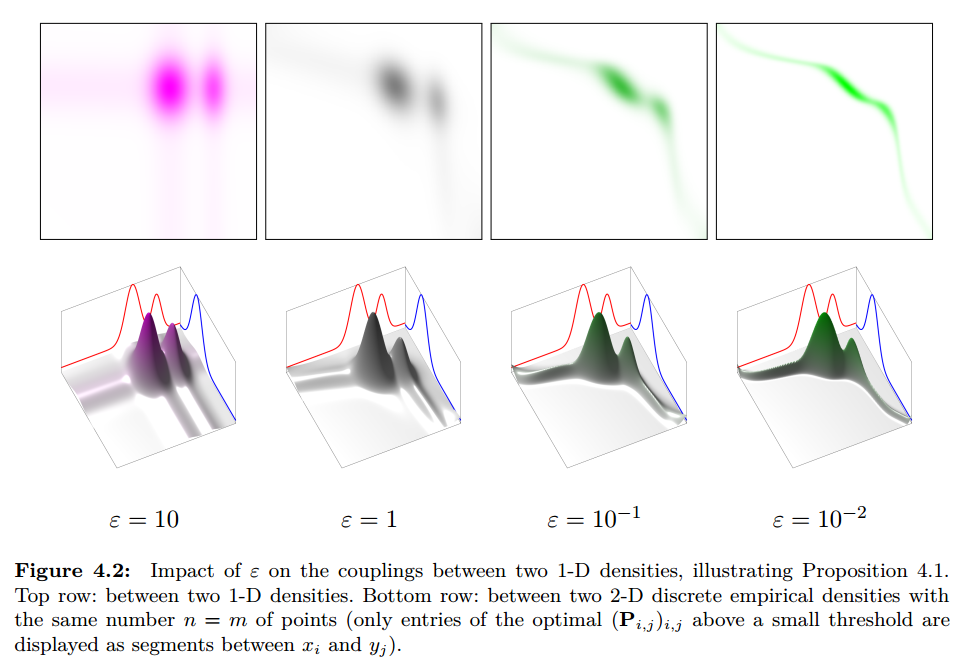
\includegraphics[scale = 0.4]{entropy_regularization2.png}}
\end{minipage}
\caption{\footnotesize{\textbf{The effect of entropy regularization on optimal coupling matrix}}}
\label{fig: entropy_regularization2}
\end{figure}

The idea of the entropic regularization of optimal transport is to use $-H$ as a regularizing function to obtain approximate solutions to the original transport problem \eqref{eqn: optimal_transport_primal}:
\begin{align}
L_{\mb{C}}^{\epsilon}(\mb{a}, \mb{b}) = \min_{\mb{P} \in U(\mb{a}, \mb{b})} \inn{\mb{P}}{\mb{C}} - \epsilon H(\mb{P}) \label{eqn: optimal_transport_primal_entropy_reg}
\end{align} This objective function is \underline{\textbf{$\epsilon$-convex}}, and thus has a unique optimal solution. The idea of adding the entropic regularization is to \textbf{diffuse} the solution to form a more \emph{"blurred"} prediction of traffic given marginals and transportation costs. Figure \ref{fig: entropy_regularization1} shows the effect of entropic regularization when $\epsilon$ is large. The entropy term pushes the optimal solution \emph{away from the boundary} to \textbf{interial point of the feasible region}.

The convergence is guaranteed 
\begin{proposition}
The unique solution $\mb{P}_{\epsilon}$ of \eqref{eqn: optimal_transport_primal_entropy_reg} converges to the optimal solution with \textbf{maximal entropy} within the set of all optimal solutions of the Kantorovich problem, namely
\begin{align}
\mb{P}_{\epsilon} \stackrel{\epsilon\rightarrow 0}{\rightarrow} \arg\min_{\mb{P}}\set{-H(\mb{P}): \;\mb{P} \in U(\mb{a}, \mb{b}),\,  \inn{\mb{P}}{\mb{C}} = L_{\mb{C}}(\mb{a}, \mb{b})}  \label{eqn: optimal_transport_primal_max_entropy}
\end{align}
so that in particular, 
\begin{align}
\lim_{\epsilon\rightarrow 0} L_{\mb{C}}^{\epsilon}(\mb{a}, \mb{b}) =  L_{\mb{C}}(\mb{a}, \mb{b})  \nonumber
\end{align}
Also we have 
\begin{align}
\lim_{\epsilon\rightarrow \infty}\mb{P}_{\epsilon} = \mb{a} \otimes \mb{b} = \mb{a}\mb{b}^{T}  \label{eqn: optimal_transport_independent}
\end{align}
\end{proposition}
We see that 
\begin{itemize}
\item For small $\epsilon >0$, the solution converges to the \textbf{maximum entropy optimal transport coupling}, as in \eqref{eqn: optimal_transport_primal_max_entropy}

\item For large $\epsilon$, however, \eqref{eqn: optimal_transport_independent} shows that the solution converges to the coupling with maximal entropy between two prescribed marginals $\mb{a}$, $\mb{b}$, namely the joint probability between \textbf{two independent random variables} distributed following $\alpha$, $\beta$. 
\end{itemize}

We also define the KL-divergence between $\mb{P}$ and the \textbf{Gibbs kernel} $\mb{K} = [\exp(-C_{i,j} / \epsilon)]$ as
\begin{align}
\kl{\mb{P}}{\mb{K}} &= \sum_{i,j}\paren{P_{i,j}\log\paren{\frac{P_{i,j}}{K_{i,j}}} - P_{i,j} + K_{i,j}}
\end{align} We can see that the unique solution $\mb{P}_{\epsilon}$ of \eqref{eqn: optimal_transport_primal_entropy_reg} is the projection of $\mb{K}$ onto the feasible region $U(\mb{a}, \mb{b})$, i.e.
\begin{align}
\mb{P}_{\epsilon} &= \min_{\mb{P} \in U(\mb{a}, \mb{b})}\kl{\mb{P}}{\mb{K}} \label{eqn: optimal_transport_primal_kl}
\end{align}

\subsection{Maximum entropy optimal transport}
We can extend this to abitrary measures using the relative entropy between $\pi$ and \textbf{product measure} $d (\alpha \otimes \beta) (x, y) = (d\alpha \otimes d\beta)(x, y)  := d\alpha(x)d\beta(y)$ and propose a regularized counterpart to \eqref{eqn: optimal_transport_primal}
\begin{align}
\cL^{\epsilon}(\alpha, \beta) :=\inf_{\pi \in U(\alpha, \beta)} \int_{\cX \times \cY} c(x, y) d \pi(x, y) + \epsilon\; \kl{\pi}{\alpha\otimes \beta} \label{eqn: optimal_transport_kl_reg_general}
\end{align} where the relative entropy is a generalization of the discrete Kullback-Leibler divergence
\begin{align}
 \kl{\pi}{\xi}  &= \int_{\cX \times \cY}\log\paren{\frac{d \pi }{d \xi} (x, y)}d\pi(x, y)  \nonumber\\
 &+  \int_{\cX \times \cY}\paren{d \xi (x, y) - d \pi (x, y)} \label{eqn: kl_divergence}
\end{align} and $\frac{d \pi }{d \xi}$ is density of $\pi$ with respect to $\xi$. The problem \eqref{eqn: optimal_transport_kl_reg_general} measure the joint probability $\pi$ again two independent probabilities $\alpha \otimes \beta$.

Using \eqref{eqn: optimal_transport_kl_reg_general} the \emph{Gibbs distributions} $\cK$, $d\cK(x,y) := \exp\paren{- \frac{c(x, y)}{\epsilon}}d\alpha(x)d\beta(y)$, we reformulate  the \emph{\textbf{maximum entropy} optimal transport problem} \eqref{eqn: optimal_transport_kl_reg_general} as
\begin{align}
\cL^{\epsilon}(\alpha, \beta) &:= \min_{\pi \in U(\alpha, \beta)} \kl{\pi}{\cK}. \label{eqn: optimal_transport_kl_reg_general2}
\end{align} As $\epsilon \rightarrow 0$, the unique solution to \eqref{eqn: optimal_transport_kl_reg_general2} converges to the maximum entropy solution $\cL(\alpha, \beta)$.

\subsection{Probability interpretation using mutual information}
The second term in \eqref{eqn: optimal_transport_kl_reg_general} is the \textbf{\emph{mutual information}} $I(X; Y) := \kl{\pi}{\alpha\otimes \beta}$. Thus we can reformulate the problem \eqref{eqn: optimal_transport_kl_reg_general} using probability interpretation
\begin{align}
\cL^{\epsilon}(\alpha, \beta) :=\min_{(X, Y) \sim \pi}& \E{(X,Y)}{c(X, Y)} + \epsilon\; I(X; Y) \label{eqn: optimal_transport_mutual_info} \\
\text{s.t. }& X\sim \alpha \nonumber\\
&Y \sim \beta \nonumber
\end{align} 

\begin{figure}
\begin{minipage}[t]{1\linewidth}
  \centering
  \centerline{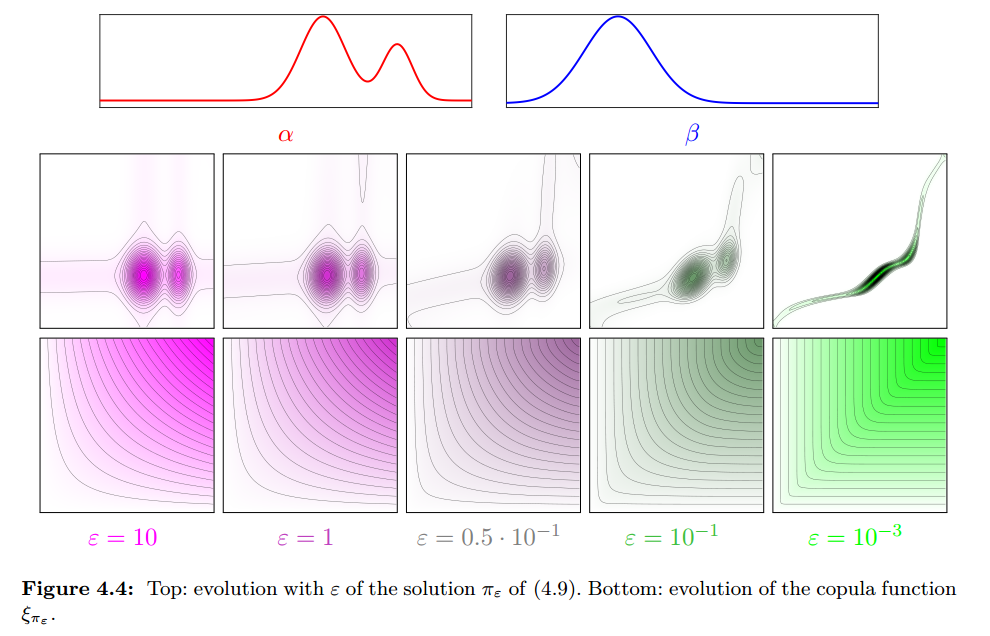
\includegraphics[scale = 0.4]{xi_epsilon.png}}
\end{minipage}
\caption{\footnotesize{\textbf{From independent to fully dependent: the change of $\xi_{\pi}$.}}}
\label{fig: xi_epsilon}
\end{figure}

A coupling $\pi \in U(\alpha, \beta)$ describes the distribution of a couple of random variables $(X, Y)$ defined on $(\cX, \cY)$, where $X \sim \alpha$ and $Y \sim \beta$. As stated in \eqref{eqn: optimal_transport_independent}, when $\epsilon\rightarrow \infty$, the algorithm minimizes the mutual information, i.e. $\pi_{\epsilon} \rightarrow \alpha \otimes \beta$. This proposes the random variables $(X, Y)$ being \textbf{independent}.  

In contrast, as $\epsilon \rightarrow 0$, $\pi_{\epsilon}$ convergence to a solution $\pi_{0}$ of the OT problem.  Note that we know for $\cX = \cY =\bR^{d}$ and $c$ is the euclidean distance, then there exists unique optimal Monge map $T$ so that $Y=T(X)$ and $X=T^{-1}(Y)$. In this case, $(X, Y)$ are in some sense \textbf{fully dependent}.

For 1-D case, we can use visualize the change of relationship between $X$ and $Y$ via changing $\epsilon$. Let the c.d.f. of $\pi$ be $F_{\pi}(x, y) = \int_{-\infty}^{x}\int_{-\infty}^{y}d\pi$ and the c.d.f of $\alpha$, $F_{\alpha}(x)$ and the c.d.f. of $\beta$, $F_{\beta}(y)$.  Specifically, we can define a function $\xi_{\pi}: \bR \rightarrow \bR$ as
\begin{align*}
\xi_{\pi}(s, t) &:= F_{\pi}(F_{\alpha}^{-1}(s), F_{\alpha}^{-1}(t)) 
\end{align*} For \emph{independent} variables, $\epsilon = +\infty$, i.e. $\pi = \alpha \otimes \beta$, one has $\xi_{\pi, \infty}(s,t) = s\,t$. In contrast, for \emph{fully dependent} variables, $\epsilon \rightarrow 0$, one has $\xi_{\pi, 0}(s, t) = \min(s, t)$. Figure \ref{fig: xi_epsilon} shows how entropic regularization generates copula $\xi_{\pi, \epsilon}$ interpolating between these two extreme cases.

\subsection{Solution of maximum entropy optimal transport}
Now we focus on solving the maximum entropy optimization problem \eqref{eqn: optimal_transport_primal_kl}
\begin{align*}
\min_{\mb{P} \in U(\mb{a}, \mb{b})} & \inn{\mb{P}}{\mb{C}} - \epsilon H(\mb{P}) \\
\Leftrightarrow \min_{\mb{P} \in U(\mb{a}, \mb{b})} & \kl{\mb{P}}{\mb{K}}
\end{align*} where $\mb{K} = \exp\paren{-\mb{C}/\epsilon}$ is the Gibbs distribution. 

The following proposition is for its solution
\begin{proposition}\label{proposition: optimal_max_entropy_primal} \citep{gabriel2019computational}
The solution to \eqref{eqn: optimal_transport_primal_entropy_reg} is \textbf{unique} and has the form
\begin{align}
\forall i\in [1:n], j\in [1:m], \quad P_{i,j} &= u_{i}\,K_{i,j}\,v_{j} \label{eqn: optimal_transport_primal_kl_sol}
\end{align} for two (unknown) scaling variable $(\mb{u}, \mb{v}) \in \bR_{+}^{n} \times \bR_{+}^{m}$.
\end{proposition}
\begin{proof}
We introduce the dual variable $\mb{\lambda}$ and $\mb{\mu}$ for each marginal constraint. The Lagrangian is 
\begin{align*}
\cL(\mb{P}, \mb{\lambda}, \mb{\mu}) := \inn{\mb{P}}{\mb{C}} - \epsilon H(\mb{P}) - \inn{\mb{\lambda}}{\mb{P}\mb{1}_{m} - \mb{a}} - \inn{\mb{\mu}}{\mb{P}^{T}\mb{1}_{n} - \mb{b}}
\end{align*} The first order condition yields
\begin{align*}
\partdiff{\cL(\mb{P}, \mb{\lambda}, \mb{\mu}) }{\mb{P}} &= \mb{C} + \epsilon \brac{\log \mb{P} } - \mb{\lambda}\mb{1}_{m}^{T} - \mb{1}_{n}\mb{\mu}^{T} =\mb{0} \\
\Leftrightarrow -\frac{1}{\epsilon}\paren{\mb{C} -  \mb{\lambda}\mb{1}_{m}^{T} - \mb{1}_{n}\mb{\mu}^{T}}  &= \log \mb{P} \\
\mb{P} &= \exp\paren{-\frac{1}{\epsilon}\paren{\mb{C} -  \mb{\lambda}\mb{1}_{m}^{T} + \mb{1}_{n}\mb{\mu}^{T}}} \\
\Leftrightarrow P_{i,j}&= \exp(\frac{\lambda_i}{\epsilon})\exp(-\frac{C_{i,j}}{\epsilon})\exp(\frac{\mu_j}{\epsilon}) := u_i K_{i,j} v_{j}
\end{align*} where the \textbf{\emph{matrix scaling factor}} $\mb{u} = [\exp(\lambda_i / \epsilon)] = \exp(\mb{\lambda}/\epsilon)$ and $\mb{v} =  [\exp(\mu_j / \epsilon)] = \exp(\mb{\mu}/\epsilon)$.\qed
\end{proof}

From \eqref{eqn: optimal_transport_primal_kl_sol}, we can write the optimal solution in \textbf{matrix form}
\begin{align}
\mb{P}^{*} &=\underline{\diag{\mb{u}}\mb{K}\diag{\mb{v}}}  \label{eqn: optimal_transport_primal_kl_sol2}
\end{align} which is a \textbf{doule stochastic matrix}.

\subsection{Dual problem for maximum entropy optimal transport}
We can find the dual problem corresponding to the primal entropic regularized optimal transport problem in \eqref{eqn: optimal_transport_primal_entropy_reg}. In particular, we have the \textbf{\emph{dual formulation}} for \emph{entropic regularized optimal transport problem}
\begin{align}
L_{\mb{C}}^{\epsilon}(\mb{a}, \mb{b}) = \max_{\mb{\lambda} \in \bR^{n}, \mb{\mu} \in \bR^{m}}& \inn{\mb{\lambda}}{\mb{a}} + \inn{\mb{\mu}}{\mb{b}} - \epsilon \inn{\exp\paren{\mb{\lambda}/\epsilon}}{\mb{K}\exp\paren{\mb{\mu}/\epsilon}} \label{eqn: optimal_transport_dual_entropy_reg}
\end{align} where $\mb{K} = \exp\paren{-\mb{C}/\epsilon}$ is the Gibbs distribution. Note that the optimal dual solution $(\mb{\lambda} , \mb{\mu})$ links to the scaling factor  $\mb{u} = \exp(\mb{\lambda}/\epsilon)$ and $\mb{v} =   \exp(\mb{\mu}/\epsilon)$ in \eqref{eqn: optimal_transport_primal_kl_sol2}.
\begin{proof}
Note that the primal optimal solution $\mb{P} = \diag{\mb{u}}\mb{K}\diag{\mb{v}}$ based on derivation in Proposition \ref{proposition: optimal_max_entropy_primal}. We substitute this into the Lagrangian function
\begin{align*}
\cL(\mb{P}, \mb{\lambda}, \mb{\mu}) &:= \inn{\mb{P}}{\mb{C}} - \epsilon H(\mb{P}) - \inn{\mb{\lambda}}{\mb{P}\mb{1}_{m} - \mb{a}} - \inn{\mb{\mu}}{\mb{P}^{T}\mb{1}_{n} - \mb{b}} \\
\Rightarrow  Q((\mb{\lambda} , \mb{\mu})& = \inn{\exp\paren{\mb{\lambda}/\epsilon}}{\paren{\mb{K}\odot \mb{C}}\exp\paren{\mb{\mu}/\epsilon}} -  \epsilon H\paren{ \diag{\exp\paren{\mb{\lambda}/\epsilon}}\mb{K}\diag{\exp\paren{\mb{\mu}/\epsilon}}}
\end{align*} For the second term, we see that 
\begin{align*}
-\epsilon H(\mb{P}) &= \inn{\mb{P}}{\log \mb{P} - \mb{1}\mb{1}^{T}}\\
&= \inn{\diag{\exp\paren{\mb{\lambda}/\epsilon}}\mb{K}\diag{\exp\paren{\mb{\mu}/\epsilon}}}{- \mb{C} +  \mb{\lambda}\mb{1}_{m}^{T} + \mb{1}_{n}\mb{\mu}^{T} - \epsilon\mb{1}\mb{1}^{T}} \\
&=- \inn{\diag{\exp\paren{\mb{\lambda}/\epsilon}}\mb{K}\diag{\exp\paren{\mb{\mu}/\epsilon}}}{\mb{C}} + \inn{\mb{\lambda}}{\mb{a}} + \inn{\mb{\mu}}{\mb{b}} - \epsilon \inn{\exp\paren{\mb{\lambda}/\epsilon}}{\mb{K}\exp\paren{\mb{\mu}/\epsilon}} \\
&= - \inn{\exp\paren{\mb{\lambda}/\epsilon}}{\paren{\mb{K}\odot\mb{C}}\exp\paren{\mb{\mu}/\epsilon}} + \inn{\mb{\lambda}}{\mb{a}} + \inn{\mb{\mu}}{\mb{b}} - \epsilon \inn{\exp\paren{\mb{\lambda}/\epsilon}}{\mb{K}\exp\paren{\mb{\mu}/\epsilon}}
\end{align*} which cancels out the first term in equation above. So we have the form of dual objective functions. \qed
\end{proof}

For arbitrary measures we have the \textbf{dual formulation} for $c: \cX \times \cY \rightarrow \bR_{+}$, constant $\epsilon >0$
\begin{align}
\sup_{(\lambda,\mu) \in \cC(\cX) \times \cC(\cY)} & \int_{\cX}\lambda d\alpha  + \int_{\cY}\mu d\beta  - \epsilon \int_{\cX \times \cY}\paren{\exp\paren{\frac{-c + \lambda \oplus \mu}{\epsilon}} - 1}d\alpha d\beta.  \label{eqn: optimal_transport_dual_entropy_reg_cont}
\end{align} where $(\lambda \oplus \mu)(x, y) = \lambda(x) + \mu(y)$.
In the case $\int_{\cX}d\alpha = 1$ and $\int_{\cY}d\beta = 1$, we have dual formulation
\begin{align}
\sup_{(\lambda,\mu) \in \cC(\cX) \times \cC(\cY)} & \int_{\cX}\lambda d\alpha + \int_{\cY}\mu  d\beta  + \text{soft-min}_{\epsilon}\set{c - \lambda \oplus \mu} \label{eqn: optimal_transport_dual_softmin_cont}
\end{align} where the soft-min operator on $f \in \cC(\cX \times \cY)$
\begin{align}
\text{soft-min}_{\epsilon}\set{f} &:= -\epsilon \int_{\cX \times \cY}\exp\paren{- f/\epsilon}d\alpha d\beta.
\end{align} As $\epsilon \rightarrow 0$, $\text{soft-min}_{\epsilon} \rightarrow \min$, as used in the unregularized and unconstrained formulation. 

The probability interpretation of dual is as below
\begin{align}
\sup_{(\lambda,\mu) \in \cC(\cX) \times \cC(\cY)} & \E{X \sim \alpha }{\lambda(X)}  + \E{Y \sim \beta}{\mu(Y)}  - \epsilon \E{X \sim \alpha, Y \sim \beta}{\exp\paren{\frac{-c(X,Y) + \lambda(X)+ \mu(Y)}{\epsilon}}}.  \label{eqn: optimal_transport_dual_entropy_prob}
\end{align}

The entropic dual \eqref{eqn: optimal_transport_dual_entropy_reg} and \eqref{eqn: optimal_transport_dual_entropy_reg_cont} is a smooth unconstrained concave maximization problem, which approximates the original Kantorovich dual \eqref{eqn: optimal_transport_dual}. The following proposition states that the optimal solution of regularized problem is still feasible for original dual problem. 
\begin{proposition}
Any pair of optimal solution to \eqref{eqn: optimal_transport_dual_entropy_reg} $(\mb{\lambda}_{*}, \mb{\mu}_{*})$ is a feasible solution to the original dual problem \eqref{eqn: optimal_transport_dual}, i.e. $(\mb{\lambda}_{*}, \mb{\mu}_{*}) \in R(\mb{C})$. For any $\epsilon >0$, 
\begin{align*}
\inn{\mb{\lambda}_{*}}{\mb{a}} + \inn{\mb{\mu}_{*}}{\mb{b}} &\le L_{\mb{C}}(\mb{a}, \mb{b}).
\end{align*}
\end{proposition}
On the other hand, a chief \textbf{advantage} of the regularized transportation cost $L_{\mb{C}}^{\epsilon}(\mb{a}, \mb{b}) $ defined in \eqref{eqn: optimal_transport_primal_entropy_reg} is that it is \emph{smooth} and \emph{convex}, which makes it a perfect fit for integrating as a loss function in variational problems.

\begin{proposition}
Given $\mb{C}$, the optimal value $L_{\mb{C}}^{\epsilon}(\mb{a}, \mb{b})$ is \underline{\textbf{convex}} function with respective to $(\mb{a}, \mb{b})$ for any $\epsilon \ge 0$. If $\epsilon >0$, then 
\begin{align}
\grad{(\mb{a}, \mb{b})}{L_{\mb{C}}^{\epsilon}(\mb{a}, \mb{b})} &= \brac{\begin{array}{c}
\mb{\lambda}_{*} \\
\mb{\mu}_{*}
\end{array}}
\end{align} where $(\mb{\lambda}_{*}, \mb{\mu}_{*})$ are the optimal solutions of regularized dual problem \eqref{eqn: optimal_transport_dual_entropy_reg} chosen so that their coordinates sum to $0$.
\end{proposition} Note that $L_{\mb{C}}^{\epsilon}(\mb{a}, \mb{b})$ is referred as \textbf{\emph{Sinkhorn divergence}} in many literature \citep{li2021hilbert}.


\subsection{Barycentric projection}
Consider the entropic regularized optimal transport problem \eqref{eqn: optimal_transport_primal_entropy_reg}. In order to obtain the map $T: \cX \rightarrow \cY$ where $\cY = \bR^{d}$, one can define the so-called \textbf{\emph{barycentric projection map}}:
\begin{align}
T: \mb{x}_{i} \in \cX \rightarrow \sum_{j}P_{i,j}y_{j} \in \cY, \label{eqn: barycentric_proj}
\end{align} where the input measures are discrete of the form $\alpha = \sum_{i=1}^{n}a_i \delta_{\mb{x}_{i}}$. Note that this map is only defined for points $\mb{x}_i$ in the support of $\alpha$. For $T$ as a permutation map, we can see that $T$ converges to the \emph{Monge map} when $\epsilon \rightarrow 0$.

Similarly, consider the arbitrary measure and optimization problem in \eqref{eqn: optimal_transport_kl_reg_general}. The solution $\pi \in U(\alpha, \beta)$ defines a density $\frac{d\pi}{d\alpha \otimes d\beta}$. The \emph{\textbf{barycentric projection map}} is defined as
\begin{align}
T: x \in \cX \rightarrow \int_{\cY}y\frac{d\pi(x, y)}{d\alpha(x) \,d\beta(y)} d\beta(y), \label{eqn: barycentric_proj_cont}
\end{align} for $\epsilon = 0$, $\pi$ is supported on the graph of the Monge map. For $\epsilon > 0$, it is a smooth map.

This map has been used in imaging. It has also been used to compute approximations of principal geodesics in the space of probability measures endowed with the Wasserstein metric.


\newpage
\section{Sinkhorn's algorithm and Its convergence}
\subsection{Sinkhorn's algorithm}
From \eqref{eqn: optimal_transport_primal_kl_sol}, we can write the optimal solution in matrix form
\begin{align}
\mb{P}^{*} &=\underline{\diag{\mb{u}}\mb{K}\diag{\mb{v}}} \nonumber
\end{align} This solution need to satisfiy the equality constrain in $U(\mb{a}, \mb{b})$: 
\begin{align}
\diag{\mb{u}}\mb{K}\diag{\mb{v}}\mb{1}_{m} = \mb{a}, \;&\; \diag{\mb{v}}\mb{K}^{T}\diag{\mb{u}}\mb{1}_{n} = \mb{b} \nonumber\\
\Rightarrow \mb{u} \odot\paren{\mb{K}\mb{v}}  = \mb{a}, \;&\; \mb{v} \odot\paren{\mb{K}^{T}\mb{u}}  = \mb{b} \label{eqn: optimal_transport_sol_condition}
\end{align} where $\odot$ means element-wise multiplication. This problem is known in the numerical analysis community as the \underline{\textbf{\emph{matrix scaling problem}}} \citep{franklin1989scaling, nemirovski1999complexity}.


\begin{figure}
\begin{minipage}[t]{1\linewidth}
  \centering
  \centerline{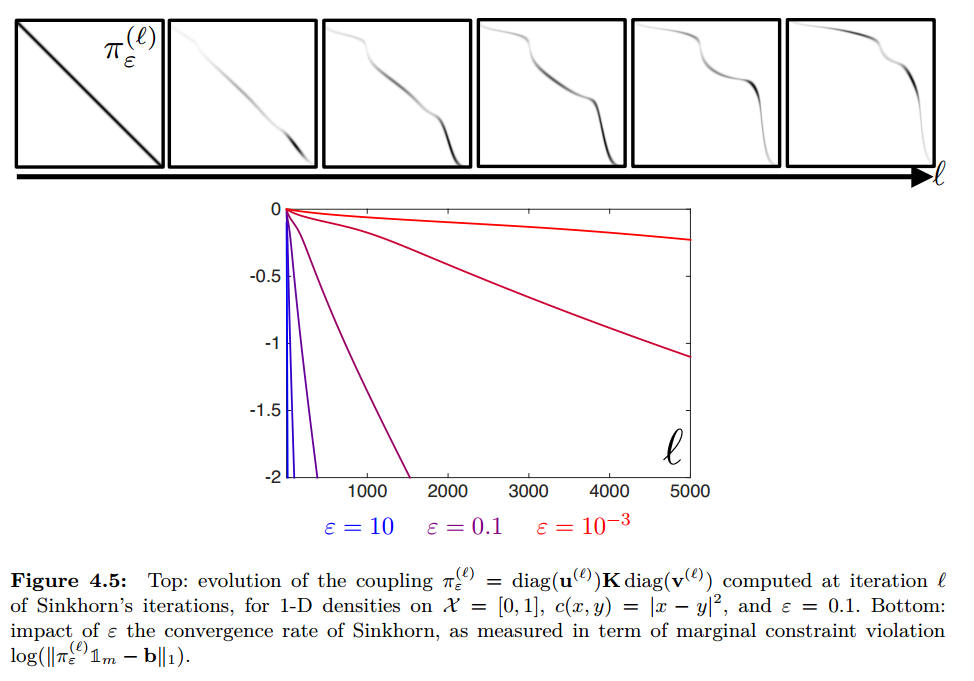
\includegraphics[scale = 0.4]{sinkhorn_update.png}}
\end{minipage}
\caption{\footnotesize{\textbf{Sinkhorn's update from Gibbs distribution to optimal transport}}}
\label{fig: sinkhorn_update}
\end{figure}

The solution $(\mb{u}, \mb{v})$ for equations \eqref{eqn: optimal_transport_sol_condition} can be obtained via two iterative updates. We have the \underline{\textbf{\emph{Sinkhorn}'s algorithm}} \citep{sinkhorn1967diagonal}
\begin{align}
\mb{u}_{t+1} &\leftarrow \frac{\mb{a}}{\mb{K}\mb{v}_{t}} := \mb{a}\oslash \mb{K}\mb{v}_{t} \label{eqn: sinkhorn_u}\\
\mb{v}_{t+1} &\leftarrow \frac{\mb{b}}{\mb{K}^{T}\mb{u}_{t+1}} :=\mb{b}\oslash \mb{K}^{T}\mb{u}_{t+1}   \label{eqn: sinkhorn_v}
\end{align} where the right hand side is element wise division i.e.  \emph{Hadamard division} ($\oslash$). Also initialized with an arbitrary positive vector $\mb{v}_{0} = \mb{1}_{m}$.  

Note that a different initialization will likely lead to a different solution for $(\mb{u}, \mb{v})$, since $(\mb{u}, \mb{v})$ are only defined up to a multiplicative constant. It turns out, however, that these iterations converge and all result in the same optimal coupling $\diag{\mb{u}}\mb{K}\diag{\mb{v}}$. Figure \ref{fig: sinkhorn_update} top row, shows the evolution of the coupling $\diag{\mb{u}_{t}}\mb{K}\diag{\mb{v}_{t}}$ computed by Sinkhorn iterations. It evolves from the Gibbs kernel $\mb{K}$ toward the optimal coupling solving  $L_{\mb{C}}^{\epsilon}(\mb{a}, \mb{b})$ by progressively shifting the mass away from the diagonal.

Note that Sinkhorn's algorithm has \textbf{advantages} in computation since it \textbf{only requires matrix-vector multiplication} and each \textbf{column} is updated \textbf{independently}. We can even combine $N$ optimal transport problems together to form matrix-matrix multiplication and update simultaneously. All of these allow it to be computed efficiently using \emph{\textbf{parallel computing}} such as GPUs. 


\subsection{Numerical analysis of Sinkhorn's algorithm}
It can be showed \citep{gabriel2019computational} that by setting $\epsilon = \frac{4 \log(n)}{\tau}$, $O(\norm{\mb{C}}{\infty}^{3}  \log(n)\tau^{-3})$ Sinkhorn iterations (with an additional rounding step to compute a valid coupling $\mb{P}' \in  U(\mb{a}, \mb{b}))$ are enough to ensure that $\inn{\mb{P}'}{\mb{C}} \le L_{\mb{C}}(\mb{a}, \mb{b}) + \tau$.  This implies that Sinkhorn computes a $\tau$-approximate solution of the unregularized OT problem in $\underline{O(n^2 \log(n)\tau^{-3})}$ operations.

Altschuler et al introduced the rounding scheme in Figure \ref{fig: sinkhorn_rounding_scheme}.
\begin{figure}
\begin{minipage}[t]{1\linewidth}
  \centering
  \centerline{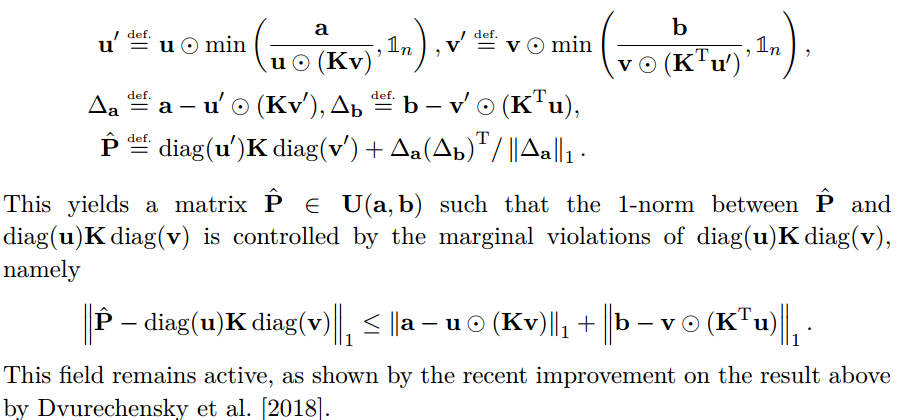
\includegraphics[scale = 0.4]{sinkhorn_rounding_scheme.png}}
\end{minipage}
\caption{\footnotesize{\textbf{Rouding scheme for Sinkhorn's algorithm}}}
\label{fig: sinkhorn_rounding_scheme}
\end{figure}

The convergence of Sinkhorn’s algorithm deteriorates as $\epsilon \rightarrow 0$. In numerical practice, however, that slowdown is rarely observed in practice. This is because Sinkhorn’s algorithm will often fail to terminate as soon as some of the elements of the kernel $\mb{K}$ become too negligible to be stored in memory as positive numbers, and
become instead null. This then affects the denominator of the updates \eqref{eqn: sinkhorn_u} and \eqref{eqn: sinkhorn_v}, causing division by $0$ error. This concern can be alleviated to some extent by carrying out computations in the \textbf{log domain}. 


\subsection{Bregman iterative projections}
Note that $U(\mb{a}, \mb{b}) = \cS_{\mb{a}}\cup \cS_{\mb{b}}$ where $\cS_{\mb{a}}= \{\mb{P}: \mb{P}\mb{1}_{m} = \mb{a}\}$ and  $\cS_{\mb{b}}= \{\mb{P}: \mb{P}^{T}\mb{1}_{n} = \mb{b}\}$. An alternative algorithm for solving problem \eqref{eqn: optimal_transport_primal_entropy_reg} is via \textbf{Bregman
iterative projections}: 
\begin{align}
\mb{P}_{t+1} &\leftarrow \text{Proj}_{\cS_{\mb{a}}}\paren{\mb{P}_{t}} :=  \arg\min_{\mb{P} \in \cS_{\mb{a}}}\kl{\mb{P}}{\mb{P}_{t}} \label{eqn: bregman_iter_a}\\
\mb{P}_{t+2} &\leftarrow \text{Proj}_{\cS_{\mb{b}}}\paren{\mb{P}_{t+1}}:=  \arg\min_{\mb{P} \in \cS_{\mb{b}}}\kl{\mb{P}}{\mb{P}_{t+1}} \label{eqn: bregman_iter_b}
\end{align} where $\text{Proj}_{\cA}(\cdot)$ is the projection via Bregman divergence (KL divergence in this case.) onto the affine set $\cA$. These iterates are equivalent to Sinkhorn iterations \eqref{eqn: sinkhorn_u} and \eqref{eqn: sinkhorn_v} since defining
\begin{align*}
\mb{P}_{2t} &= \diag{\mb{u}_{t}}\mb{K}\diag{\mb{v}_{t}}\\
\Rightarrow \mb{P}_{2t+1} &= \diag{\mb{u}_{t+1}}\mb{K}\diag{\mb{v}_{t}}\\
\Rightarrow \mb{P}_{2t+2} &= \diag{\mb{u}_{t+1}}\mb{K}\diag{\mb{v}_{t+1}}
\end{align*}
In practice, however, one should prefer using \eqref{eqn: sinkhorn_u} and \eqref{eqn: sinkhorn_v}, which only requires \emph{manipulating \textbf{scaling} \textbf{vectors}} and \emph{\textbf{multiplication} against a \textbf{Gibbs kernel}}, which can often be accelerated.

\subsection{Proximal point algorithm}
In order to approximate a solution of the original unregularized ($\epsilon = 0$) problem \eqref{eqn: optimal_transport_primal}, it is possible to use \emph{\textbf{iteratively} the Sinkhorn algorithm}, using the so-called \underline{\textbf{proximal point algorithm}} for the KL metric.

Denote the unconstrained objective function as
\begin{align*}
F(\mb{P}) := \inn{\mb{P}}{\mb{C}} + \ind{\mb{P} \in U(\mb{a}, \mb{b}) }
\end{align*}

The \textbf{\emph{proximal point iterations}} for the KL divergence computes a minimizer of $F$
\begin{align}
\mb{P}_{t+1} &\leftarrow \text{Proj}_{F(\mb{P})}\paren{\mb{P}_{t}} :=  \arg\min_{\mb{P} \in \bR_{+}^{n\times m}}\kl{\mb{P}}{\mb{P}_{t}} + \frac{1}{\epsilon}F(\mb{P}) \label{eqn: proximal_point_iterations}
\end{align} The proximal point algorithm is the most basic \emph{proximal splitting method}. Initially introduced for the Euclidean metric, it extends to any Bregman divergence, so in particular it can be applied here for the KL divergence. 

The optimization appearing in \eqref{eqn: proximal_point_iterations} is very similar
to the entropy regularized problem \eqref{eqn: optimal_transport_primal_entropy_reg}, with the relative entropy $\kl{\cdot}{\mb{P}_{t}}$ used in
place of the negative entropy $-H$.  Since the optimal solution for each subproblem is of similar form,  we can still use the Sinkhorn algorithm, with $\mb{K} := \exp(-\frac{1}{\epsilon}\mb{C})\odot \mb{P}_{t}$. Iterations \eqref{eqn: proximal_point_iterations} can thus be implemented by \textbf{running the Sinkhorn algorithm at each iteration}. Assuming for simplicity $\mb{P}_{0} = \mb{1}_{n}\mb{1}_{m}^{T}$, these iterations thus
have the form
\begin{align*}
\mb{P}_{t+1} &= \diag{\mb{u}_{t}\odot \ldots \odot \mb{u}_{0}}\brac{\exp(-\frac{1}{\epsilon/(1+t)}\mb{C})\odot \mb{P}_{t}}\diag{\mb{v}_{t}\odot \ldots \odot \mb{v}_{0}}
\end{align*} Here the kernel is  $\exp(-\frac{1}{\epsilon/(1+t)}\mb{C})$ and the temperature of the kernel decays with parameter $\epsilon/t$. This method is thus
tightly connected to a series of works which combine Sinkhorn with some \textbf{decaying schedule} on the regularization.


\subsection{Convergence analysis of Sinkhorn's algorithm}
The analysis used a metric called \textbf{Hilbert projective metric}. 
\begin{definition}
The \textbf{\emph{Hilbert metric}}, also known as the \textbf{\emph{Hilbert projective metric}}, is an explicitly defined distance function on a \emph{bounded convex subset} of the $n$-dimensional Euclidean space $\bR^n$.

For the space of positive vectors $\bR_{+, *}^{n} \subset \bR^{n}$,  Hilbert projective metric on $\bR_{+, *}^{n}$
\begin{align*}
d_{\cH}(\mb{u}, \mb{v}) &= \log \max_{i,j}\frac{u_i v_j}{u_j v_i} \quad \forall \mb{u}, \mb{v} \in \bR_{+, *}^{n} \\
&= \norm{\log \mb{u} - \log \mb{v}}{\text{var}},
\end{align*} where $\norm{ \mb{f} }{\text{var}} = \max f_{i} - \min f_{i}$.  It can be shown to be a distance on the \emph{\textbf{projective cone}} $ \bR_{+, *}^{n}/ \sim$, where $\mb{u} \sim \mb{v}$ means that $\exists r > 0, \mb{u} = r\mb{v}$. This means that $d_{\cH}$ satisfies the triangular inequality and $d_{\cH}(\mb{u}, \mb{v}) = 0$ if and only if $\mb{u} \sim \mb{v}$. 
\end{definition}

\begin{theorem}(\textbf{Global linear convergence}) \citep{franklin1989scaling}\\
For Sinkhorn algorithm, one has $(\mb{u}_{t}, \mb{v}_{t}) \rightarrow (\mb{u}_{*}, \mb{v}_{*})$ and 
\begin{align}
d_{\cH}(\mb{u}_{t}, \mb{u}_{*}) = O(\lambda(\mb{K})^{2t}) \quad & \quad d_{\cH}(\mb{v}_{t}, \mb{v}_{*}) = O(\lambda(\mb{K})^{2t})  \label{eqn: convergence_sinkhorn0}
\end{align} where $\lambda(\mb{K}) := \frac{\sqrt{\eta(\mb{K})} - 1}{\sqrt{\eta(\mb{K})} + 1} $ and $\eta(\mb{K}) =\max_{i,j,k,l} \frac{K_{i,k} K_{j,l}}{K_{j,k} K_{i,l}}$

One also has 
\begin{align}
d_{\cH}(\mb{u}_{t}, \mb{u}_{*}) &\le \frac{d_{\cH}(\mb{P}_{t}\mb{1}_{m}, \mb{a})}{1- \lambda(\mb{K})^2}, \label{eqn: convergence_sinkhorn1}\\
d_{\cH}(\mb{v}_{t}, \mb{v}_{*}) &\le \frac{d_{\cH}(\mb{P}_{t}^{T}\mb{1}_{n}, \mb{b})}{1- \lambda(\mb{K})^2} \nonumber
\end{align} where we denoted $\mb{P}_{t} =\diag{\mb{u}_{t}}\mb{K}\diag{\mb{v}_{t}}$. Last, one has
\begin{align}
\norm{\log \mb{P}_{t} - \log \mb{P}_{*}}{\infty} & \le d_{\cH}(\mb{u}_{t}, \mb{u}_{*}) + d_{\cH}(\mb{v}_{t}, \mb{v}_{*})  \label{eqn: convergence_sinkhorn2}
\end{align} where $\mb{P}_{*}$ follows \eqref{eqn: optimal_transport_primal_kl_sol} is the unique solution of \eqref{eqn: optimal_transport_primal_entropy_reg}.
\end{theorem}

\begin{figure}
\begin{minipage}[t]{1\linewidth}
  \centering
  \centerline{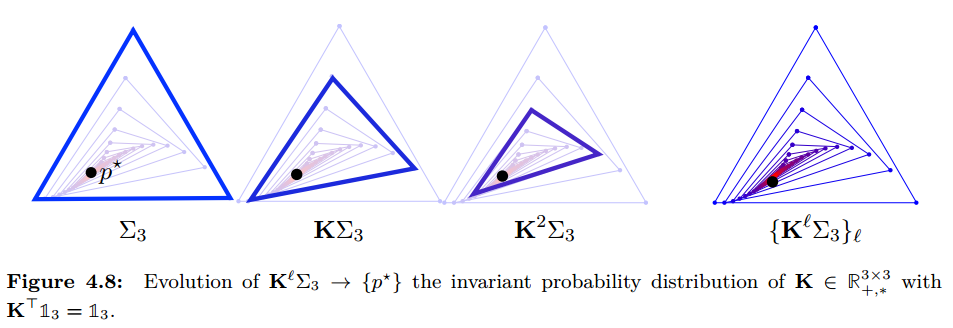
\includegraphics[scale = 0.42]{sinkhorn_boundary.png}}
\end{minipage}
\caption{\footnotesize{\textbf{Evolution of boundary of $\mb{K}_t \Delta_{3}$}}}
\label{fig: sinkhorn_boundary}
\end{figure}


\subsection{Log-domain Sinkhorn to solve the dual problem}
Recall the dual objective function
\begin{align}
Q(\mb{\lambda}, \mb{\mu}) &:= \inn{\mb{\lambda}}{\mb{a}} + \inn{\mb{\mu}}{\mb{b}} - \epsilon \inn{\exp\paren{\mb{\lambda}/\epsilon}}{\mb{K}\exp\paren{\mb{\mu}/\epsilon}}  \label{eqn: optimal_transport_dual_entropy_reg_obj}
\end{align}

\subsubsection{Sinkhorn as block coordinate ascent in dual domain}
A simple approach to solving the unconstrained maximization problem \eqref{eqn: optimal_transport_dual_entropy_reg} is to use an exact \emph{\textbf{block coordinate ascent}} strategy, namely to update alternatively $\mb{\lambda}$ and $\mb{\mu}$ to cancel the respective gradients in these variables of the objective of \eqref{eqn: optimal_transport_dual_entropy_reg}. 

The gradient of dual objective w.r.t $\mb{\lambda}$ and $\mb{\mu}$ are
\begin{align}
\partdiff{Q(\mb{\lambda}, \mb{\mu})}{\mb{\lambda}} &= \mb{a} - \epsilon\, \exp\paren{\mb{\lambda}/\epsilon}\odot \paren{\mb{K}\exp\paren{\mb{\mu}/\epsilon}}   \label{eqn: ent_reg_dual_obj_grad_lambda} \\
\partdiff{Q(\mb{\lambda}, \mb{\mu})}{\mb{\mu}} &= \mb{b} - \epsilon\, \exp\paren{\mb{\mu}/\epsilon}\odot \paren{\mb{K}^{T}\exp\paren{\mb{\lambda}/\epsilon}}   \label{eqn: ent_reg_dual_obj_grad_mu}
\end{align} 

Thus \underline{\textbf{\emph{block coordinate ascent in dual domain}}} can therefore be implemented in a closed form by applying successively the following updates, starting from any arbitrary $\mb{\mu}_{0}$,
Solving the equation $\partdiff{Q(\mb{\lambda}, \mb{\mu})}{\mb{\lambda}} = \mb{0}$ and $\partdiff{Q(\mb{\lambda}, \mb{\mu})}{\mb{\mu}} = \mb{0}$, the updated on $\mb{\lambda}$ and on $\mb{\mu}$, respectively are obtained
\begin{align}
\mb{\lambda}_{t+1} &\leftarrow \arg\min_{\mb{\lambda}}Q(\mb{\lambda}, \mb{\mu}_{t})\nonumber\\
&= \epsilon \log \mb{a} - \epsilon \log\paren{\mb{K}\exp\paren{\mb{\mu}_{t}/\epsilon}} \label{eqn: block_coordinate_ascent_dual_lambda}\\
\mb{\mu}_{t+1} &\leftarrow  \arg\min_{\mb{\mu}}Q(\mb{\lambda}_{t+1}, \mb{\mu})\nonumber\\
&= \epsilon \log \mb{b} - \epsilon \log\paren{\mb{K}^{T}\exp\paren{\mb{\lambda}_{t+1}/\epsilon}}  \label{eqn: block_coordinate_ascent_dual_mu}
\end{align} Such iterations are mathematically equivalent to the Sinkhorn iterations \eqref{eqn: sinkhorn_u} and \eqref{eqn: sinkhorn_v} when considering the primal-dual relations highlighted in $\mb{u} = \exp(\mb{\lambda}/\epsilon)$ and $\mb{v} =   \exp(\mb{\mu}/\epsilon)$. Indeed, we recover that at any iteration
\begin{align*}
(\mb{\lambda}_{t}, \mb{\mu}_{t}) &= \epsilon(\log \mb{u}_{t}, \log \mb{v}_{t})
\end{align*}

\subsubsection{Log-domain Sinkhorn}
Note that the second term in \eqref{eqn: block_coordinate_ascent_dual_lambda}
\begin{align*}
 -\epsilon[\log\paren{\mb{K}\exp\paren{\mb{\mu}_{t}/\epsilon}}]_{i,j} &= -\epsilon\log\paren{\sum_{j}\exp(-\paren{C_{i,j} -  \mu_{j, t}}/\epsilon)} \\
 &:= \text{soft-min}_{\epsilon}\paren{\brac{\mb{C} -  \mb{1}_{n}\mb{\mu}_{t}^{T}}_{i}} = \text{soft-min}_{\epsilon, \text{row}}\paren{\mb{C} -  \mb{1}_{n}\mb{\mu}_{t}^{T}}
\end{align*} actually choose the \emph{\textbf{soft-min}} of difference $C_{i,j} - \mu_{j, t}$ over index $j$, where the \textbf{soft-min operator}
\begin{align*}
\text{soft-min}_{\epsilon}(\mb{z}) &:= -\epsilon \log \sum_{i}\exp\paren{-\mb{z}_i/\epsilon}.
\end{align*} These operations are equivalent to the entropic c-transform. 
Using this notation, \textbf{Sinkhorn’s iterates} \eqref{eqn: block_coordinate_ascent_dual_lambda} and \eqref{eqn: block_coordinate_ascent_dual_mu} read 
\begin{align}
\mb{\lambda}_{t+1} &\leftarrow  \text{soft-min}_{\epsilon, \text{row}}\set{\mb{C} -\mb{1}_{n}\mb{\mu}_{t}^{T}} +  \epsilon\log \mb{a} \\
\mb{\mu}_{t+1} &\leftarrow  \text{soft-min}_{\epsilon, \text{column}}\set{\mb{C} - \mb{\lambda}_{t+1}\mb{1}_{m}^{T}} + \epsilon \log \mb{b} 
\end{align} Here, we introduce the \emph{\textbf{log-sum-exp} stabilization} trick to avoid underflow for small values of $\epsilon$. That trick suggests that we subtract the minimum term in the soft-min operator:
\begin{align*}
\text{min}_{\epsilon}(\mb{z}) &:= \bar{z} -\epsilon \log \sum_{i}\exp\paren{-(\mb{z}_i -   \bar{z})/\epsilon}
\end{align*} Instead of substracting $ \bar{z}:=\min_{i}z_{i}$ to stabilize the log-domain iterations as above, one can actually substract the previously computed scalings. This leads to the \emph{stabilized} iteration. The \underline{\textbf{log-domain}} \textbf{\emph{Sinkhorn algorithm}} is described as below:
\begin{align}
\mb{\lambda}_{t+1} &\leftarrow  \mb{\lambda}_{t} + \text{soft-min}_{\epsilon, \text{row}}\set{\mb{C}- \mb{\lambda}_{t}\mb{1}^{T} - \mb{1}\mb{\mu}_{t}^{T} } +  \epsilon\log \mb{a} \label{eqn: log_domain_dual_sinkhorn_lambda}\\
\mb{\mu}_{t+1} &\leftarrow \mb{\mu}_{t} +  \text{soft-min}_{\epsilon, \text{column}}\set{\mb{C} - \mb{\lambda}_{t+1}\mb{1}^{T}- \mb{1}\mb{\mu}_{t}^{T}} + \epsilon \log \mb{b} \label{eqn: log_domain_dual_sinkhorn_mu}
\end{align} where $\text{soft-min}_{\epsilon}(\mb{z}) = -\epsilon \log \sum_{i}\exp\paren{-\mb{z}_i/\epsilon}$ is the soft-min operator. The notation $\text{soft-min}_{\epsilon, \text{row}}$ means that we take soft-min for each row of matrix of $\bR^{n\times m}$ and returning a column of size $n$. 

In contrast to the original iterations \eqref{eqn: sinkhorn_u} and  \eqref{eqn: sinkhorn_v}, these log-domain iterations \eqref{eqn: log_domain_dual_sinkhorn_lambda} and \eqref{eqn: log_domain_dual_sinkhorn_mu} are stable for arbitrary $\epsilon > 0$, because the quantity $S(\mb{\lambda},\mb{\mu}) := \mb{C} - \mb{\lambda}_{t+1}\mb{1}^{T}- \mb{1}\mb{\mu}_{t}^{T}$ stays bounded during the iterations. 

The \textbf{downside} is that it requires $nm$ computations of exp at each step. Computing a $\text{soft-min}_{\epsilon, \text{row}}$ or $\text{soft-min}_{\epsilon, \text{column}}$  is typically substantially \underline{\textbf{\emph{slower}}} than matrix multiplications and requires computing line by line soft-minima of matrices $\mb{S}$.  There is therefore \emph{no efficient way} to parallelize the application of Sinkhorn maps for several marginals \emph{simultaneously}.

\subsection{Sinkhorn divergence}
\begin{definition}(\textbf{Sinkhorn divergences}) \citep{cuturi2013sinkhorn, gabriel2019computational}.\\
Let $(\mb{\lambda}_{*}, \mb{\mu}_{*})$ be optimal solutions to dual problemm \eqref{eqn: optimal_transport_dual_entropy_reg} and $\mb{P}_{*}$ be the solution to primal problem \eqref{eqn: optimal_transport_primal_entropy_reg}. The \emph{Wasserstein distance} is approximated using the following \textbf{primal} and \textbf{dual Sinkhorn divergences}:
\begin{align}
\mathfrak{P}_{\mb{C}}^{\epsilon}(\mb{a}, \mb{b}) &:= \inn{\mb{P}_{*}}{\mb{C}} = \inn{\exp\paren{\mb{\lambda}/\epsilon}}{(\mb{K}\odot \mb{C})\exp\paren{\mb{\mu}/\epsilon}} \label{eqn: sinkhorn_primal_divg}\\
\mathfrak{D}_{\mb{C}}^{\epsilon}(\mb{a}, \mb{b}) &:=\inn{\mb{\lambda}_{*}}{\mb{a}} + \inn{\mb{\mu}_{*}}{\mb{b}} \label{eqn: sinkhorn_dual_divg}
\end{align} where $\odot$ stands for the elementwise product of matrices.
\end{definition}

\begin{proposition}
The following relationship holds:
\begin{align}
\mathfrak{D}_{\mb{C}}^{\epsilon}(\mb{a}, \mb{b}) \le L_{\mb{C}}^{\epsilon}(\mb{a}, \mb{b})   \le \mathfrak{P}_{\mb{C}}^{\epsilon}(\mb{a}, \mb{b})  \label{eqn: sinkhorn_primal_dual_divg_inequality}
\end{align}
Furthermore
\begin{align}
 \mathfrak{P}_{\mb{C}}^{\epsilon}(\mb{a}, \mb{b})  - \mathfrak{D}_{\mb{C}}^{\epsilon}(\mb{a}, \mb{b}) & = \epsilon (H(\mb{P}_{*})- 1) \label{eqn: sinkhorn_primal_dual_divg_gap}
\end{align}
\end{proposition}
\begin{proof}
By definition of optimality, we have
\begin{align*}
L_{\mb{C}}^{\epsilon}(\mb{a}, \mb{b}) =  \mathfrak{P}_{\mb{C}}^{\epsilon}(\mb{a}, \mb{b}) -  \epsilon H(\mb{P}_{*})  \le    \mathfrak{P}_{\mb{C}}^{\epsilon}(\mb{a}, \mb{b})\\
L_{\mb{C}}^{\epsilon}(\mb{a}, \mb{b}) =   \mathfrak{D}_{\mb{C}}^{\epsilon}(\mb{a}, \mb{b})  - \epsilon \inn{\exp\paren{\mb{\lambda}_{*}/\epsilon}}{\mb{K}\exp\paren{\mb{\mu}_{*}/\epsilon}} \ge  \mathfrak{D}_{\mb{C}}^{\epsilon}(\mb{a}, \mb{b})
\end{align*}
Thus 
\begin{align*}
 \mathfrak{P}_{\mb{C}}^{\epsilon}(\mb{a}, \mb{b})  - \mathfrak{D}_{\mb{C}}^{\epsilon}(\mb{a}, \mb{b}) & =\epsilon H(\mb{P}_{*}) -  \epsilon \inn{\exp\paren{\mb{\lambda}_{*}/\epsilon}}{\mb{K}\exp\paren{\mb{\mu}_{*}/\epsilon}}\\
 &=  \epsilon (H(\mb{P}_{*}) - 1) 
\end{align*}
 Note that 
\begin{align*}
\inn{\exp\paren{\mb{\lambda}_{*}/\epsilon}}{\mb{K}\exp\paren{\mb{\mu}_{*}/\epsilon}} &= \sum_{i}\sum_{j}e^{\lambda_{i,*}/\epsilon}e^{-C_{i,j}/\epsilon}  e^{\mu_{j,*}/\epsilon} \\
&= \sum_{i}\sum_{j}e^{(\lambda_{i,*} +\mu_{j,*} - C_{i,j} )/\epsilon} \\
&= \sum_{i}\sum_{j}P_{i,j, *} = 1 \quad (\text{by K.K.T condition. see \eqref{eqn: optimal_transport_primal_kl_sol}})
\end{align*} \qed
\end{proof} 


\begin{proposition} (Finite Sinkhorn divergences).\\
For finite Sinkhorn iterations:
\begin{align}
\mathfrak{D}_{\mb{C}}^{(t)}(\mb{a}, \mb{b}) &:=\inn{\mb{\lambda}_{t}}{\mb{a}} + \inn{\mb{\mu}_{t}}{\mb{b}} \label{eqn: sinkhorn_dual_divg_finite}
\end{align}
The following relationship holds:
\begin{align}
\mathfrak{D}_{\mb{C}}^{(t)}(\mb{a}, \mb{b}) \le L_{\mb{C}}^{\epsilon}(\mb{a}, \mb{b})    \label{eqn: sinkhorn_finite_dual_divg_inequality}
\end{align}
\end{proposition}
Note that during the Sinkhorn iterations, $(\mb{\lambda}_{t}, \mb{\mu}_{t})$ is still dual feasbile for \eqref{eqn: optimal_transport_dual_entropy_reg}. Therefore the inequality holds. Note that the primal iteration $\mb{P}_{t}$ is not primal feasible, since, by definition, these iterates are designed
to satisfy upon convergence marginal constraints.

Unlike the regularized expression $L_{\mb{C}}^{\epsilon}(\mb{a}, \mb{b})$, the finite Sinkhorn divergence $\mathfrak{D}_{\mb{C}}^{(t)}(\mb{a}, \mb{b}) $ is \underline{\textbf{not}}, in general, a \underline{\textbf{convex}} function of its arguments (this can be easily checked numerically). $\mathfrak{D}_{\mb{C}}^{(t)}(\mb{a}, \mb{b})$ is, however, a \emph{\textbf{differentiable} function} which can be differentiated using \textbf{automatic differentiation} techniques with respect to any of its arguments, notably $\mb{C}$, $\mb{a}$, or $\mb{b}$.

Note in many literatures, we have the following definition of Sinkhorn divergence:
\begin{definition} \citep{li2021hilbert}\\
The \textbf{\emph{Sinkhorn divergence}} is formally defined as: 
\begin{align}
\cL^{\epsilon}(\alpha, \beta) :=\inf_{\pi \in U(\alpha, \beta)} \int_{\cX \times \cY} c(x, y) d \pi(x, y) + \epsilon\; \kl{\pi}{\alpha\otimes \beta}
\end{align}
In \citep{vialard2019elementary}, it is defined as
\begin{align*}
\cL^{\epsilon}(\alpha, \beta) + \frac{1}{2}\paren{\cL^{\epsilon}(\alpha, \gamma) + \cL^{\epsilon}(\gamma, \beta)}
\end{align*}
\end{definition}
\newpage
\bibliographystyle{plainnat}
\bibliography{book_reference.bib}
\end{document}